\documentclass[11pt]{article}
\usepackage[utf8]{inputenc}
\usepackage[english]{babel}
\usepackage{amsmath}
\usepackage{dsfont}
\usepackage{graphicx}
\usepackage{float}
\usepackage{lipsum}
\usepackage{multicol}
\usepackage{xcolor}
\usepackage{tabularx}
\usepackage{booktabs}
\usepackage{hyperref}
\usepackage{wrapfig}

\newcolumntype{Y}{>{\centering\arraybackslash}X}
\usepackage[left=2.00cm, right=2.00cm, top=2.00cm, bottom=2.00cm]{geometry}

\title{AN2DL Reports Template}

\begin{document}
    
    \begin{figure}[H]
        \raggedright
        
\includegraphics[scale=0.4]{figures/polimi.png} \hfill 
\includegraphics[scale=0.3]{figures/airlab.jpeg}
    \end{figure}
    
    \vspace{5mm}
    
    \begin{center}
        % Select between First and Second
        {\Large \textbf{AN2DL - First Homework Report}}\\
        \vspace{2mm}
        % Change with your Team Name
        {\Large \textbf{DeepL}}\\
        \vspace{2mm}
        % Team Members Information
        {\large Matteo Bonfadini,}
        {\large Elena Lippolis,}
        {\large Lorenzo Cossiga,}
        {\large Michele Baggi}\\
        \vspace{2mm}
        % Codabench Nicknames
        {50mgk,}
        {elenali,}
        {lorenzocossiga,}
        {mik01}\\
        \vspace{2mm}
        % Matriculation Numbers
        {243786,}
        {252310,}
        {242309,}
        {252119}\\
        \vspace{5mm}
        \today
    \end{center}    
    \vspace{5mm}
    
    \begin{multicols*}{2}        
        \section{Introduction}

        The project aims to implement \textit{multi-class image classification} using \textbf{deep learning} techniques for blood cell analysis. This \textit{supervised learning} task requires balancing model complexity to ensure generalization to unseen data while minimizing \textit{overfitting}. The primary \textbf{goal} is to design a solid neural network that classifies blood cells into the correct categories with high accuracy.
        
        The \textbf{approach} involves dataset analysis to identify potential issues such as class imbalance, image quality, and the need for preprocessing. We then developed simple deep learning models to establish a performance benchmark, which was subsequently refined into more complex models. We applied techniques such as data augmentation, transfer learning, and fine-tuning to improve model accuracy and generalization and to reduce overfitting. By following this approach, we were able to develop a classification model for blood cells.
        
        \section{Problem Analysis}

        The \textbf{dataset} consists of 13759 RGB images designed for the classification of different types of blood cells. Each image has size 96x96 pixels and it is labeled with one of eight (from 0 to 7) classes, representing the following blood cell types: basophils (0), eosinophils (1), erythroblasts (2), immature granulocytes (3), lymphocytes (4), monocytes (5), neutrophils (6), and platelets (7). We show in Figure~\ref{fig:dataset} a sample for each class.

        \begin{figure}[H]
            \centering
            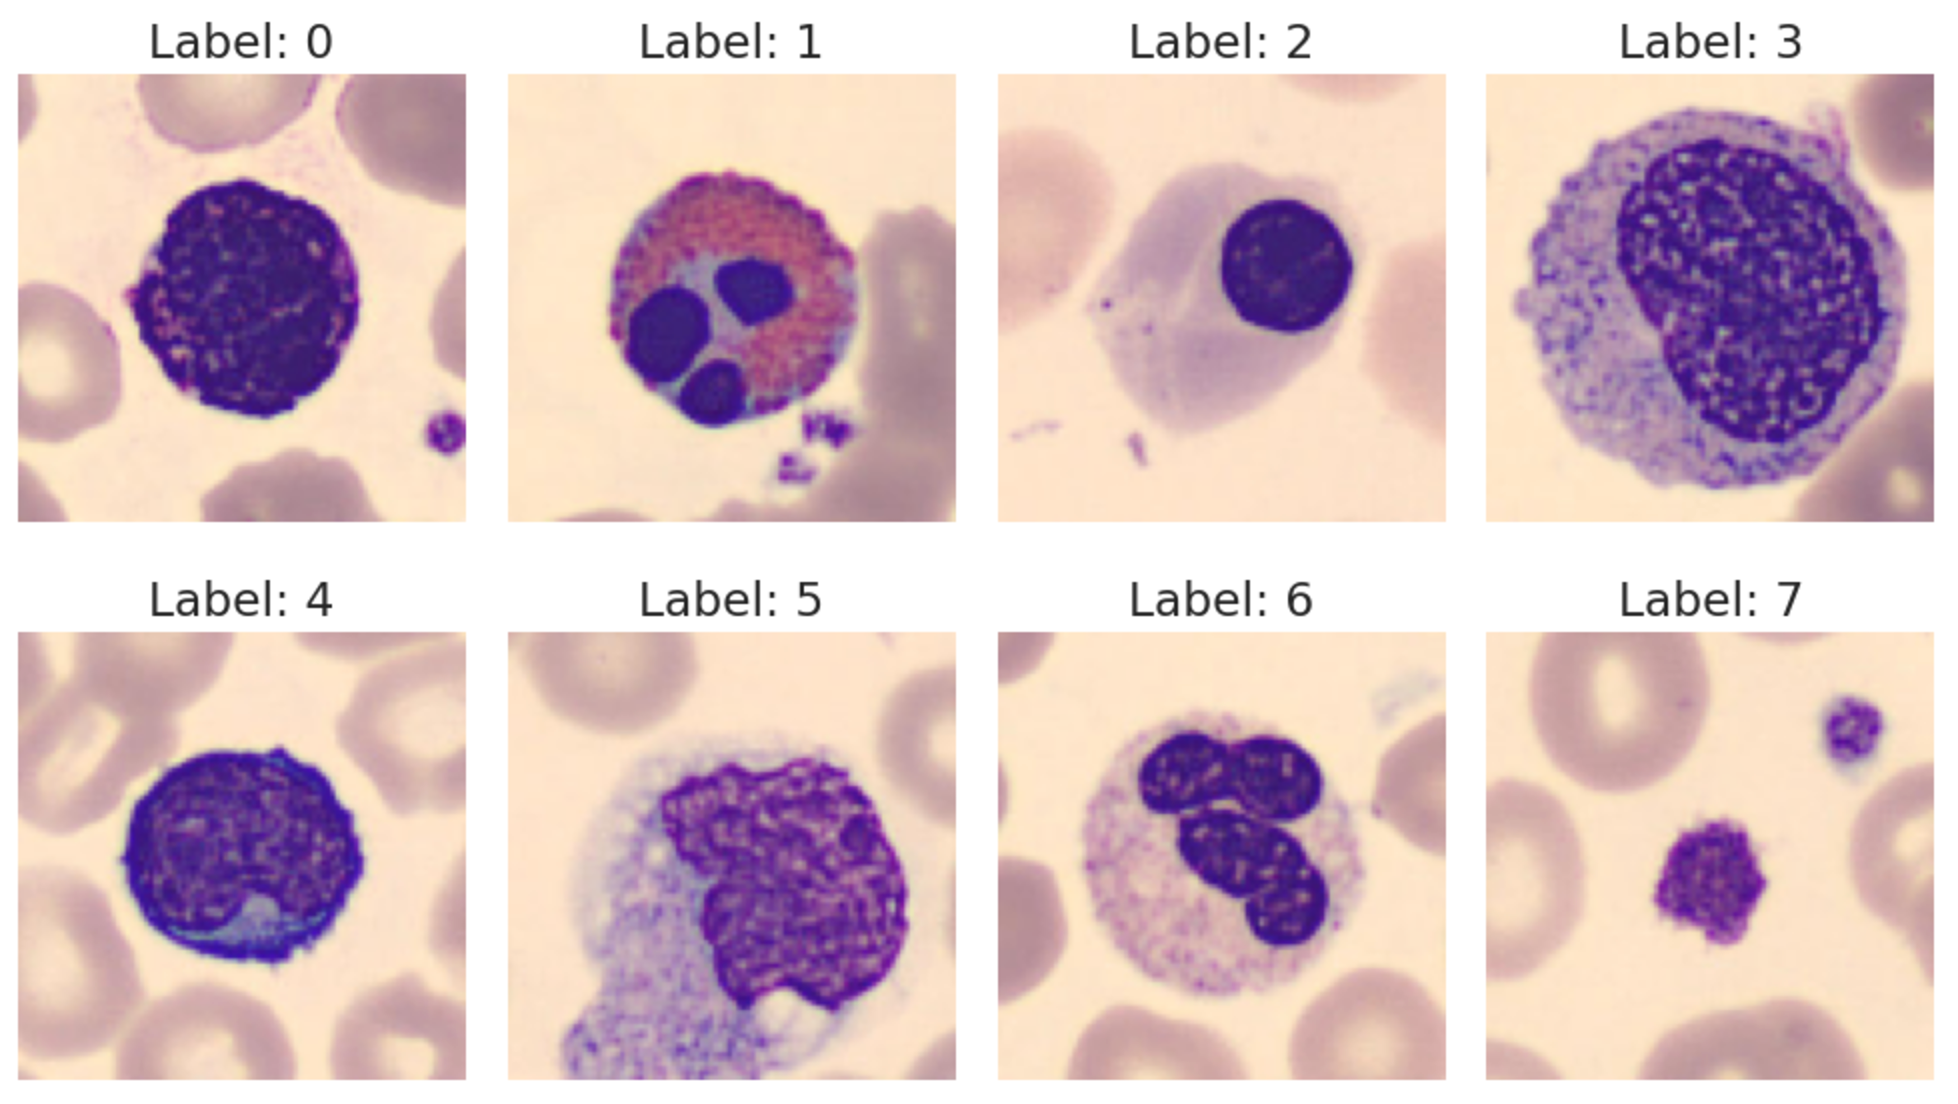
\includegraphics[width=\linewidth]{figures/SCR-20241122-nvwz.png}
            \caption{Example of an image for each class}
            \label{fig:dataset}
        \end{figure}

        We tackled the problem in a 3-phase approach.

        \subsection{Phase 1: Data Inspection}

        Firstly, we inspected the dataset and printed its shape, as shown in Table~\ref{tb:class-shape}. Secondly, a deeper inspection revealed the presence of \textit{obvious} outliers, as shown in Figure~\ref{fig:rickroll}, which could skew the learning process: 200 samples of the very same blood cell for each class and 200 rick roll. Therefore we proceed by erasing those images.

        We also noticed some images with grayscale backgrounds, but further analysis through \textit{PCA} based on the Mahalanobis distance \cite{outliers} (normalizing the dataset) showed this pattern did not negatively influence our performance. This indicates that the grayscale background images do not impact the model's ability to learn effectively. 

        \begin{table}[H]
            \centering
            \setlength{\tabcolsep}{1pt}
            \caption{Shape of the dataset.}
            \begin{tabularx}{\linewidth}{lYY}
                \toprule
                & Class & Number of samples \\
                \midrule
                & 0 & 1052  \\
                & 1 & 2381  \\
                & 2 & 1285  \\
                & 3 & 2226  \\
                & 4 & 1049  \\
                & 5 & 1393  \\
                & 6 & 2530  \\
                & 7 & 1843  \\
                \midrule
                Total: & \textbf{8}  & \textbf{13759} \\
                \bottomrule
            \end{tabularx}
            \label{tb:class-shape}
        \end{table}

        \begin{figure}[H]
            \centering
            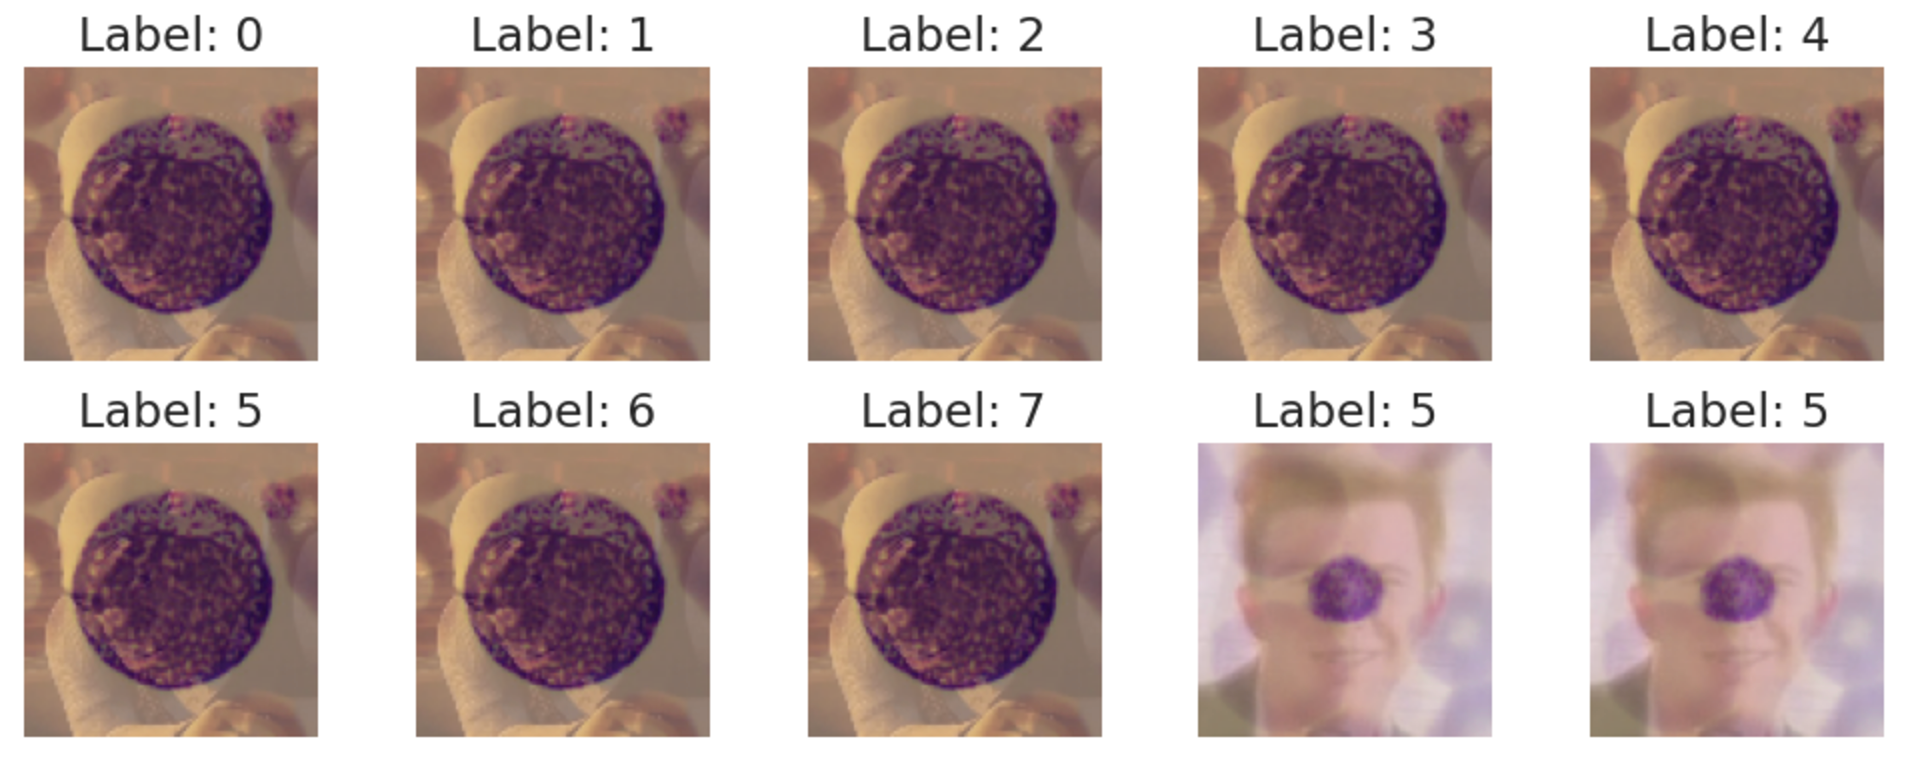
\includegraphics[width=\linewidth]{figures/SCR-20241122-oigg.png}
            \caption{Samples of \textit{obvious} outliers.}
            \label{fig:rickroll}
        \end{figure}

        \subsection{Phase 2: Class Imbalance}

        The new dataset, for a total of \textbf{11959} blood cell images, has shape reported in Figure~\ref{fig:imbalance}.

        \begin{figure}[H]
            \centering
            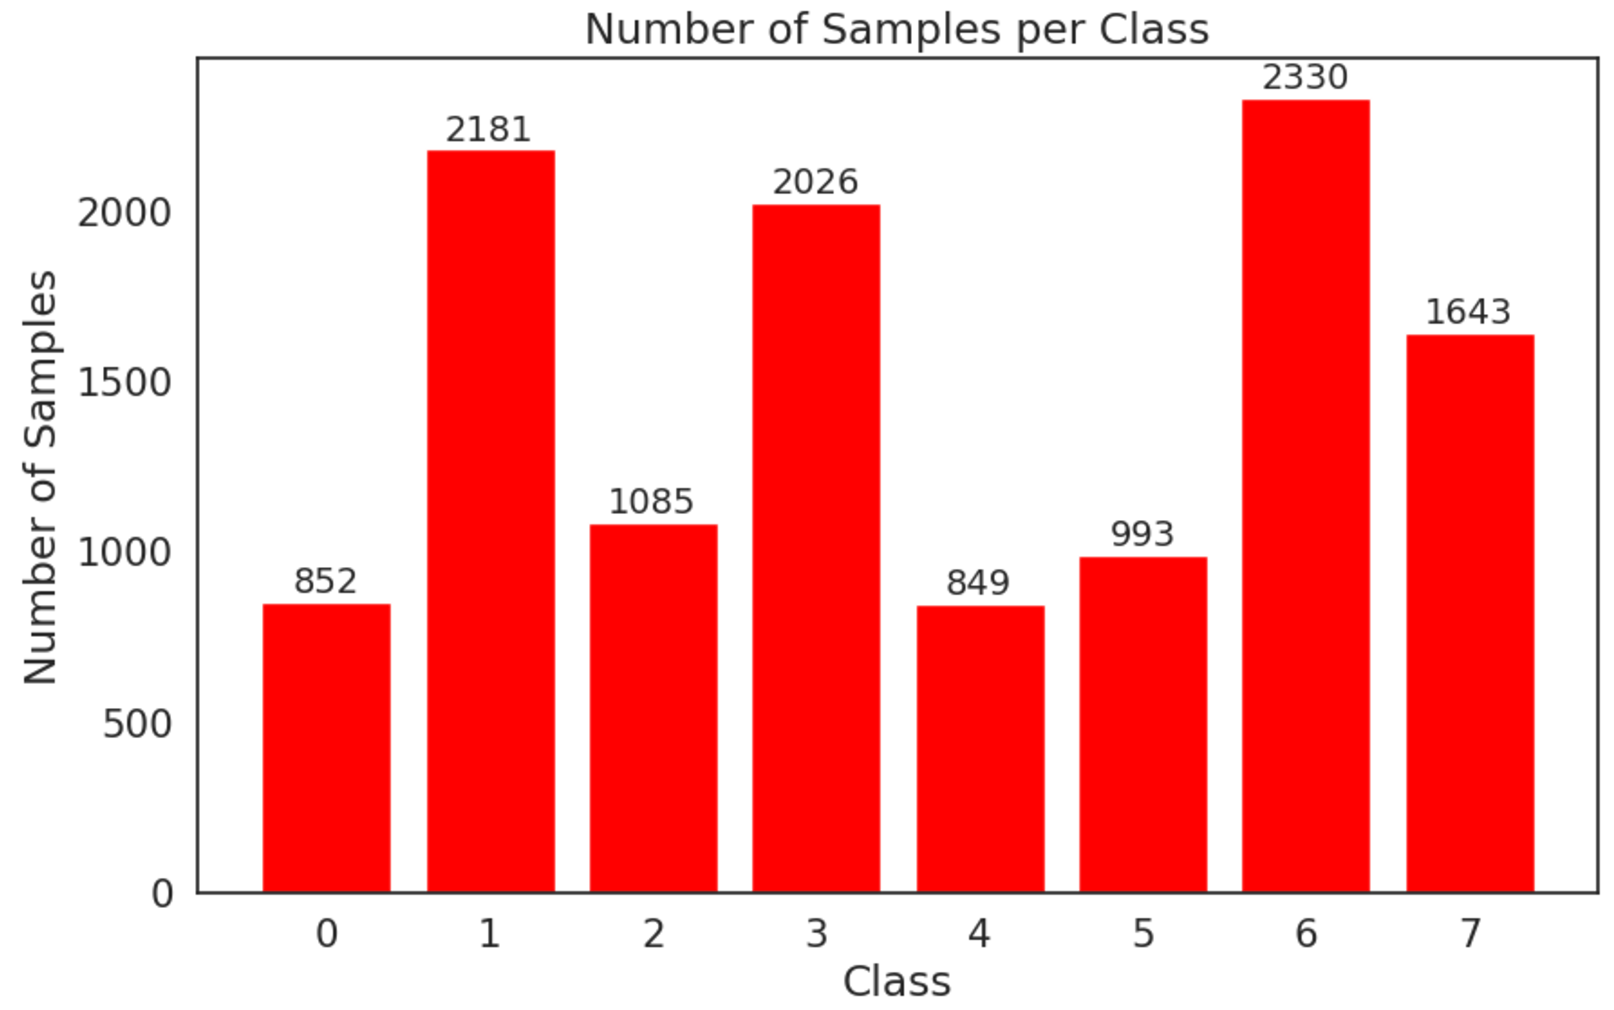
\includegraphics[width=0.75\linewidth]{figures/SCR-20241122-ooty.png}
            \caption{Number of samples in each class.}
            \label{fig:imbalance}
        \end{figure} 

        Upon closer inspection, one might observe that the dataset exhibits class imbalance. This problem poses additional challenges for training a model that generalizes effectively across all categories.

        To address this, after the splitting of the dataset into training, validation and test sets according to an 83:13:4 ratio, we balanced the training one by replicating images in the underrepresented classes. The result is a new training set with 2000 images for each class.

        Finally, we applied \textbf{data augmentation techniques} to create variations of these images (\textit{oversampling}) \cite{oversampling}. In particular, after trials and errors, we decided to use \texttt{AugMix} and \texttt{RandAugment} \cite{aug}.

        \subsection{Phase 3: Mixed Precision}

        One of the main \textbf{challenges} we encountered was the low training speed, which was solved by implementing mixed precision \cite{mixed-precision}. This technique uses lower precision (16-bit floating point numbers) for computations while retaining single precision (32-bit) for weight updates. Mixed precision accelerated training and reduced energy consumption, all while maintaining a reasonable accuracy level. Additionally, overfitting of the training set reduced the model's ability to perform well on unseen (and possibly \textit{modified}) test data. However, we intentionally allowed initial overfitting assuming that we needed to verify that the model was able to fit the training data before addressing generalization issues, to employ only later techniques like early stopping and dropout layers to mitigate overfitting and enhance performance on unseen data \cite{overfitting}.

        \subsection{Assumptions}

        We \textbf{assumed} the dataset to be solid, with minimal labeling error or inconsistencies beyond the identified outliers. Moreover, we hypothesized that a simple baseline model would provide reasonable performance before moving to more complex architectures and that some overfitting was necessary at first, and we would have to address it later. 

        The last assumption we made was that Codabench would not let us down when we needed it to test our final models ... apparently that was a bit too much to ask for.

        \begin{figure}[H]
            \centering
            
\includegraphics[width=0.3\linewidth]{meme/Screenshot from 2024-11-21 11-03-01.png}
        \end{figure}

        \section{Method}

        The task suggests to use Categorical Cross-Entropy as loss function. If $y_{ij}$ is the output probability of class $j$ for observation $i$, then:
        \begin{equation*}
        \label{eq:loss}
        \operatorname{Loss}(y_{\text{pred}},y_{\text{true}}) = - \frac{1}{N} \sum_{i=1}^N \sum_{j=1}^J y_{\text{true},ij} \log(y_{\text{pred},ij})
        \end{equation*}
        where $N$ is the number of samples and $J = 12$ is the number of classes.

        As metric we used Accuracy as requested:
        \begin{equation*}
        \label{eq:accuracy}
        \operatorname{Accuracy} = \frac{1}{N} \sum_{i=1}^N \mathds{1}_{[\operatorname{argmax}_j (y_{\text{pred},ij}) = \operatorname{argmax}_j (y_{\text{true},ij})]}
        \end{equation*}

        In addition, we also considered the F1--score per class to better understand the weaknesses of the model.

        \begin{center}
        \begin{tabular}{c}
        \hline
        Layer\\
        Layer\\
        Dense(128)\\
        BatchNormalization\\
        Dropout\\
        \hline
        \end{tabular}
        \end{center}

        \section{Experiments}
        For your experiments, you might want to present your results in tables. Here's an example of a wide table comparing different models:

        \begin{table*}[H]
            \centering
            \setlength{\tabcolsep}{3pt}
            \caption{An example of wide table. Best results are highlighted in \textbf{bold}.}
            \begin{tabularx}{\textwidth}{lYYYc}
                \toprule
                Model & Accuracy & Precision & Recall & ROC AUC\\
                \midrule
                VGG18         &  72.20 $\pm$ 3.06    &   94.95 $\pm$ 0.52     &   86.95 $\pm$ 0.55    &   80.16 $\pm$ 0.81\\
                Custom Model        &  27.71 $\pm$ 3.19    &   75.70 $\pm$ 1.07     &   55.75 $\pm$ 2.16    &   36.60 $\pm$ 1.26\\
                ResNet18    &  \textbf{89.24 $\pm$ 2.38}    &   \textbf{95.54 $\pm$ 0.49}     &   \textbf{93.43 $\pm$ 1.30}    &   \textbf{91.68 $\pm$ 0.71}\\
                \bottomrule
            \end{tabularx}
            \label{tab:Performance}
        \end{table*}

        \noindent For more specific measurements, you might use a narrower table:
    
        \begin{table}[H]
            \centering
            \setlength{\tabcolsep}{3pt}
            \caption{An example of table. Best results may be highlighted in \textbf{bold}.}
            \begin{tabularx}{\linewidth}{lY}
                \toprule
                Time [$\mu$s] & Distance [mm]\\
                \midrule
                22$\pm$4 & 8$\pm$1\\
                17$\pm$3 & 7$\pm$1\\
                15$\pm$3 & 6$\pm$1\\
                13$\pm$2 & 5$\pm$1\\
                10$\pm$2 & 4$\pm$1\\
                8$\pm$2 & 3$\pm$1\\
                5$\pm$1 & 2$\pm$1\\
                37$\pm$1 & 1$\pm$1\\
                \bottomrule
            \end{tabularx}
            \label{tb:Measurements}
        \end{table}

        \noindent You can also include figures to visualise your results:
        \begin{figure}[H]
            \centering
            
\includegraphics[width=0.75\linewidth]{figures/random.jpeg}
            \caption{Example figure showing [describe what the figure shows]}
            \label{fig:results}
        \end{figure}

        \noindent Reference figures using like:``As shown in Figure~\ref{fig:results}..."

        \section{Results}
        Present your main findings here. You might want to:
        \begin{itemize}
            \item Compare your results with baselines
            \item Highlight key achievements using \textbf{bold text}
            \item Explain any unexpected outcomes
        \end{itemize}

        \section{Discussion}
        In this section, analyse your results critically. Consider:
        \begin{itemize}
            \item Strengths and weaknesses
            \item Limitations and assumptions
        \end{itemize}

        \section{Conclusions}
        Summarise your work and discuss potential future directions. This is where you can:
        \begin{itemize}
            \item Restate main contributions
            \item Suggest improvements
            \item Propose future work
        \end{itemize}

        \newpage

        \section{Logbooks}

        Here we can write our personal logbooks.

        \subsection{Matteo}

        \begin{itemize}
            \item \href{https://drive.google.com/drive/folders/1XqCxOkXIFV81NU8IlltS38bM65k9N-bR?usp=sharing}{Google Drive folder}
            \item \href{https://github.com/BonfaTex/DeepL-1}{\LaTeX{} repository}
            \item A bit of data inspection and noised aumentation
        \end{itemize}

        \subsection{Lorenzo}

        \begin{itemize}
            \item 
        \end{itemize}

        \subsection{Michele}

        \begin{itemize}
            \item 
        \end{itemize}

        \subsection{Elena}

        \begin{itemize}
            \item 
        \end{itemize}

        \newpage

        \section{Intro}
    
        \begin{itemize}
            \item This project focuses on image classification about blood cells
            \item goal: create network to recognize blood cells
            \item approach: understand the dataset and its problems, start with simple models, discover augmentation \& class balance, transfer learning, fine tuning
        \end{itemize}
    
        \section{Problem analysis} 
    
        \begin{itemize}
            \item Dataset characteristics: presenza di ovvi outlier (200 x classe + 200 rick roll classe 5), classi non bilanciate
            \item Main challenges: lentezza allenamento (mixed precision), problemi di generalizzazione al test set (overfitting), codabench
            \item Initial assumptions: che il codabench non funzionava; 
        \end{itemize}

        \section{Method} 
        \begin{itemize}
            \item Bilanciamento classic
            \item augmentation
            \item modello (VGG16)
            \item fine tuning
        \end{itemize}
        References:
        \begin{itemize}
            \item Use of VGG16 on medical images: \cite{guan2019vgg16}, \cite{acevedo2019bloodcells}
            \item Balance of classes through replication
            \item Lecture 5: Facing Overfitting, October 2: "A good practice for designing neural networks: train a model that overfits the data. This ensures the model has enough complexity (e.g. sufficient layers, neurons, and parameters) to solve the problem effectively. At this stage, generalization is not the focus: it's about verifying that the model is capable of fitting the training data. Once overfitting is confirmed, techniques like early stopping and dropout layers are introduced to prevent overfitting and improve generalization to unseen data."
        \end{itemize}

        \bibliography{references}
        
        \bibliographystyle{abbrv}
    
    \end{multicols*}







\end{document}